\documentclass[12pt]{article}
\usepackage[margin=1in]{geometry} 
\usepackage{graphicx}
\usepackage{amsmath,amsthm,amssymb}
\usepackage{hyperref}
\usepackage{tikz}

\title{
    \textbf{Theory Assignment 4} \\ 
    \textbf{CS5280} \\
}

\author{
    \textbf{Darpan Gaur} \\
    \textbf{CO21BTECH11004}
}


\date{}

\begin{document}
\maketitle

\hrulefill

\section*{Problem 5.2}
\begin{equation*}
    m = w_0(x_0) w_0(y_0) c_0 r_1(x_0) w_1(x_1) r_2(x1) w_2(y_2) w_1(y_1) w_2(x_3)
\end{equation*}
Conisder the following version order on the variables:
\begin{equation*}
    x_0 \ll x_1 \ll x_3, \quad y_0 \ll y_1 \ll y_2
\end{equation*}
Building the MVSG(m, $\ll$) we have the following edges:
\begin{itemize}
    \item $r_1(x_0) \implies t_0 \rightarrow t_1$
    \item $r_2(x_1) \implies t_1 \rightarrow t_2$
    \item $r_2(x_1), w_3(x_3)$ and $ x_2 \ll x_3 \implies t_2 \rightarrow t_3$
    \item $r_1(x_0), w_3(x_3)$ and $ x_0 \ll x_3 \implies t_1 \rightarrow t_3$
\end{itemize}
\begin{figure}[h]
    \centering
    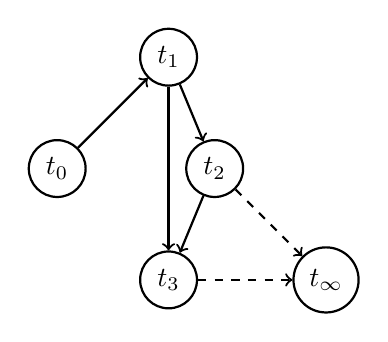
\begin{tikzpicture}[node distance={2cm}, thick, main/.style = {draw, circle}]
        \node[main] (0) {$t_0$};
        \node[main] (1) [above right of=0] {$t_1$};
        \node[main] (2) [right of=0] {$t_2$};
        \node[main] (3) [below right of=0] {$t_3$};
        \node[main] (4) [below right of=2] {$t_\infty$};
    
        \path[->] (0) edge node {} (1);
        \path[->] (1) edge node {} (2);
        \path[->] (2) edge node {} (3);
        \path[->] (1) edge node {} (3);
        \path[->, dashed] (3) edge node {} (4);
        \path[->, dashed] (2) edge node {} (4);
        
    \end{tikzpicture}
    \caption{MVSG for m}
    \label{fig:mvsg}
\end{figure}
In figure \ref{fig:mvsg}, we see that MVSG is acyclic. Appropriate version for $t_\infty$ is $x_3$ and $y_2$, i.e., $r_\infty(x_3), \quad r_\infty(y_2)$.

\section*{Problem 5.6}
\begin{equation*}
    m = w_1(x) c_1 r_2(x) r_3(x) c_2 r_4(x) w_3(x) c_4 c_3
\end{equation*}
Figure \ref{fig:mvto} shows the execution of m under MVTO protocol.\\
Here $w_3(x_3)$ step is rejected because $r_4(x_1)$ has already been scheduled, such that $ts(t_1) < ts(t_3) < ts(t_4)$. Hence, transaction $t_3$ is aborted, as it creates a new version $x_3$, however transaction $t_4$ has already read the version $x_1$. \\
\begin{figure}[h]
    \centering
    \begin{tikzpicture}
        \node at (-0.5, 0) {\(t_1\)};
        \draw[-] (0,0) -- (2, 0);
        \draw[line width=0.75mm] (0, -0.25) -- (0, 0.25);

        \draw[-] (1, -0.25) -- (1, 0.25);
        \node[below] at (1, -0.2)  {\(w_1(x_1)\)};

        \draw[line width=0.75mm] (2, -0.25) -- (2, 0.25);

        \node at (2, -1.25) {\(t_2\)};
        \draw[-] (2.5, -1.25) -- (4.5, -1.25);
        \draw[line width=0.75mm] (2.5, -1.5) -- (2.5, -1);

        \draw[-] (3, -1.5) -- (3, -1.0);
        \node[below] at (3, -1.55)  {\(r_2(x_1)\)};

        \draw[line width=0.75mm] (4.5, -1.5) -- (4.5, -1);
        
        \node at (3, -2.5) {\(t_3\)};
        \draw[-] (3.5, -2.5) -- (8.5, -2.5);
        \draw[line width=0.75mm] (3.5, -2.75) -- (3.5, -2.25);
        
        \draw[-] (4.25, -2.75) -- (4.25, -2.25);
        \node[below] at (4.25, -2.8)  {\(r_3(x_1)\)};

        \draw[-] (7, -2.75) -- (7, -2.25);
        \node[below] at (7, -2.8)  {\(w_3(x_3)\)};

        \draw[line width=0.75mm] (8.5, -2.75) -- (8.5, -2.25);
        \node at (9.5, -2.5) {\(abort\)};

        \node at (4.5, -3.75) {\(t_4\)};
        \draw[-] (5, -3.75) -- (7.7, -3.75);
        \draw[line width=0.75mm] (5, -4) -- (5, -3.5);
        \draw[-] (6, -4) -- (6, -3.5);
        \node[below] at (6, -4.05)  {\(r_4(x_1)\)};
        
        \draw[line width=0.75mm] (7.7, -4) -- (7.7, -3.5);


    \end{tikzpicture}
    \caption{m execution under MVTO protocol}
    \label{fig:mvto}
\end{figure}

\section*{Problem 5.9}
The proposed protocol is nor correct and does not guarantee MVSR schedules. \\
Consider the following schedule:
\begin{equation*}
    m = w_0(x_0) w_0(y_0) c_0 r_1(x_0) r_1(y_0) r_2(x_0) r_2(y_0) w_1(x_1) c_1 w_2(y_2) c_2
\end{equation*}
Consider the following version order on the variables: $x_0 \ll x_1, \quad y_0 \ll y_2$\\
Building the MVSG(m, $\ll$) we have the following edges:
\begin{itemize}
    \item $r_1(x_0) \implies t_0 \rightarrow t_1$
    \item $r_2(x_0), w_1(x_1)$ and $x_0 \ll x_1 \implies t_2 \rightarrow t_1$
    \item $r_1(y_0), w_2(y_2)$ and $y_0 \ll y_2 \implies t_1 \rightarrow t_2$
\end{itemize}
Figure \ref{fig:mvsg_q3} shows the MVSG for m. As graph is cyclic, hence m is not in MVSR.\\
\begin{figure}[h]
    \centering
    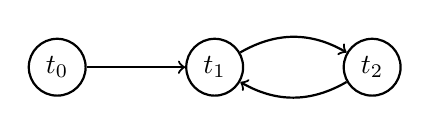
\begin{tikzpicture}[node distance={2cm}, thick, main/.style = {draw, circle}]
        \node[main] (0) {$t_0$};
        \node[main] (1) [right of=0] {$t_1$};
        \node[main] (2) [right of=1] {$t_2$};
    
        \path[->] (0) edge node {} (1);
        \path[->] (1) edge [bend left] node {} (2);
        \path[->] (2) edge [bend left] node {} (1);
    
    \end{tikzpicture}
    \caption{MVSG for m}
    \label{fig:mvsg_q3}
    
\end{figure}

\end{document}


